\definecolor{code_comment}{RGB}{200, 200, 200}
\definecolor{code_keyword}{RGB}{150, 50, 200}

\lstset{
  backgroundcolor=\color{lightgray},
  basicstyle=\small\ttfamily,
  keywordstyle=\bfseries\ttfamily\color{code_keyword},
  stringstyle=\color{red}\ttfamily,
  commentstyle=\color{code_comment}\ttfamily,
  emph={comment},
  showstringspaces=false,
  flexiblecolumns=false,
  tabsize=4,   
  xleftmargin=15pt
}

\begin{lstlisting} [caption={ein paar Zeilen code}\label{lst:test123},captionpos=t,language=JAVA] 
public class Main
{
	static int main(String[] args)
	{
    	System.out.println("hello world!"); // comment
    	return 0;
    }
}
\end{lstlisting}

% EntityBuffer Image
\begin{wrapfigure}{r}{0.3\linewidth}
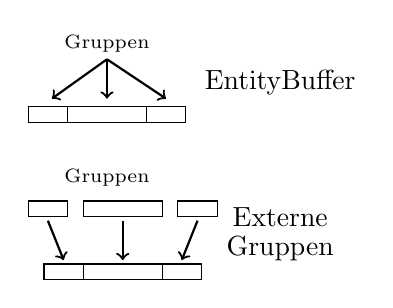
\begin{tikzpicture}
\node at (3.2, 0.5) {EntityBuffer};

\draw (0, 0) rectangle (2, 0.2);
\draw (0.5, 0) -- (0.5, 0.2);
\draw (1.5, 0) -- (1.5, 0.2);
\scriptsize
\node at (1, 1) {Gruppen};
\draw [thick,->] (1, 0.8) -- (0.3, 0.3);
\draw [thick,->] (1, 0.8) -- (1, 0.3);
\draw [thick,->] (1, 0.8) -- (1.75, 0.3);

\normalsize
\node at (3.2, -1.2) {Externe};
\node at (3.2, -1.6) {Gruppen};

\draw (0.2, -2) rectangle (2.2, -1.8);
\draw (0.7, -2) -- (0.7, -1.8);
\draw (1.7, -2) -- (1.7, -1.8);
\scriptsize
\node at (1, -0.7) {Gruppen};
\draw (0,-1) rectangle (0.5, -1.2);
\draw (0.7,-1) rectangle (1.7, -1.2);
\draw (1.9,-1) rectangle (2.4, -1.2);

\draw [thick,->] (0.25, -1.25) -- (0.45, -1.75);
\draw [thick,->] (1.2, -1.25) -- (1.2, -1.75);
\draw [thick,->] (2.15, -1.25) -- (1.95, -1.75);
\end{tikzpicture}
\end{wrapfigure}
